%%
%% This is file `sample-sigconf.tex',
%% generated with the docstrip utility.
%%
%% The original source files were:
%%
%% samples.dtx  (with options: `sigconf')
%% 
%% IMPORTANT NOTICE:
%% 
%% For the copyright see the source file.
%% 
%% Any modified versions of this file must be renamed
%% with new filenames distinct from sample-sigconf.tex.
%% 
%% For distribution of the original source see the terms
%% for copying and modification in the file samples.dtx.
%% 
%% This generated file may be distributed as long as the
%% original source files, as listed above, are part of the
%% same distribution. (The sources need not necessarily be
%% in the same archive or directory.)
%%
%% The first command in your LaTeX source must be the \documentclass command.
\documentclass[sigconf, nonacm, natbib, screen, balance=False]{acmart}

% Documentation for packages
% - ACM Article Template
%    https://www.acm.org/publications/proceedings-template
% - Pseudocode typesetting CLRS-style:
%    https://www.cs.dartmouth.edu/~thc/clrscode/clrscode3e.pdf
% - Python code typesetting
%    http://ctan.uib.no/macros/latex/contrib/listings/listings.pdf
% - AMS Math
%    http://ctan.uib.no/macros/latex/required/amsmath/amsldoc.pdf
% - Graphics
%    http://ctan.uib.no/macros/latex/required/graphics/grfguide.pdf

\usepackage{clrscode3e}  
\usepackage{listings}
\usepackage[capposition=top]{floatrow}
\usepackage{placeins}
\usepackage[utf8]{inputenc}


\lstset{language=Python, basicstyle=\ttfamily}

% based on https://tex.stackexchange.com/questions/279240/float-for-lstlisting
\usepackage{float}
\usepackage{subcaption,graphicx}
\floatstyle{ruled}
\newfloat{listing}{tbph}{lop}
\floatname{listing}{Listing}
\def\lstfloatautorefname{Listing} % needed for hyperref/auroref

\citestyle{acmauthoryear}

%% end of the preamble, start of the body of the document source.
\begin{document}

\title{Benchmarking sorting algorithms in Python}
\subtitle{INF221 Term Paper, NMBU, Autumn 2020}

\author{Anders Mølmen Høst and Muhammad Fahad ljaz}
\affiliation{Data Science Section, Faculty of Science and Technology,
  Norwegian University of Life Sciences}
\email{anders.molmen.host@nmbu.no, muhammad.fahad.ijaz@nmbu.no}

%% The abstract is a short summary of the work to be presented in the
%% article.
\begin{abstract}
ABSTRACT TEXT
\vspace
\end{abstract}

%%
%% This command processes the author and affiliation and title
%% information and builds the first part of the formatted document.
\maketitle

\section{Introduction}\label{sec:intro}

The purpose of this paper is to perform benchmarks on various sorting algorithms. Benchmarking is to be done on test data of different size and structure to analyse the behaviors of the algorithms in each case.Those differences are to be visualised graphically and the results are analysed. The results are important to find out the real life behavior of the algorithm as compared to their theoretically expected behaviour.The following sorting algorithms were analysed based on the psuedocode presented in the course.
\begin{itemize}
\item Quadratic algorithms
    \begin{itemize}
    \item Insertion Sort
    \item Bubble Sort
    \end{itemize}
\item Sub-quadratic algorithms
    \begin{itemize}
    \item Merge Sort
    \item Quick Sort
    \end{itemize}
\item Combined Algorithm
    \begin{itemize}
    \item Merge Sort switching to insertion sort for small data
    \end{itemize}
\item Built-in sorting functions
    \begin{itemize}
    \item Python 'sort()'
    \item NumPy 'sort()'
    \end{itemize}
\end{itemize}

\vspace



\section{Theory}\label{sec:theory}

\subsection{Quadratic algorithms}\label{sec:quadratic-algorithms}

\subsubsection{Insertion-sort}\label{sec:quadratic-algorithms}
Insertion sort uses in incremental approach to sorting. It builds the sorted array by taking only one item at a time. It starts by comparing the first two elements of the array. If there are already sorted, it will move onto the next set. Otherwise, it'll swap them. Then it will compare the second element with the third one and swap them if necessary. If swapped, it'll then compare the new second element with the first and swap them if required. In the next step, it'll compare the the third and the fourth elements and repeat the same process for each element until all the sorted.
Insertion sort will give best performance on an array which is already sorted. The worst case would be an array which is sorted in reverse order.
Insertion sort is an in-place sorting algorithm.
    
\subsubsection{Bubble sort}\label{sec:quadratic-algorithms}
Bubble sort sorts in the following way. It starts with the last positioned element of the array. Then compares the last element with the second last element. If the last element is smaller, the elements swap positions in the array. Continuing with the second last element. This element is then compared to the third last element and the process is repeated until all adjacent elements are compared. Now the smallest element of the array are placed in the first position. Then during the next round we start with the last element again and comparing adjacent elements and stop when the second element is reached. Now we have the two smallest numbers in their correct positions. The process continues until all elements are sorted.

The run time of the algorithm has an upper bound of $O(n^2)$ in the worst case. Bubble sort will need to swap all elements while iterating through the inner loop. Then after each iteration through the outer loop the remaining elements to sort will only go down by one. In the best case the run time is $O(n)$ since the algorithm then only iterates through the list one time and will not make any swaps. However the average case is $O(n^2)$. Because of the double for-loops the algorithm will need to compare and possible swap elements, sorting one element at each iteration.
The algorithm sorts in place as Insertion sort, so that the elements are not copied in a new array requiring additional storage space.

\begin{listing}
  % Pseudocode caption above the code.
  \caption{Bubble sort algorithm from \citet[Ch.~2. p 40 ]{CLRS_2009}.}
  \label{lst:bubble_algo}
  %
  % For documentation on how to typeset CLRS-style pseudocode, see
  % https://www.cs.dartmouth.edu/~thc/clrscode/clrscode3e.pdf
  % 
\begin{codebox}
\Procname{$\proc{Bubble-sort}(A)$}
\li \For $i = 1$ \To $A.length - 1$
\li \Then \For $j = A.length$ \Downto $i + 1$
\li \Then \If $A[j] < A[j-1]$
\li \Then exchange $A[j]$ with $A[j-1]$
\End
\end{codebox}
\end{listing}
\FloatBarrier

\subsection{Sub-quadratic algorithms}\label{sec:sub-quadratic-algorithms}

\subsubsection{Merge-sort}\label{sec:merge-sort}
Merge sort uses the divide-and-conquer approach which is a recursive approach to sorting. The approach is to divide the problem into several sub problems and then solve them recursively. Then it combines the results of the sub problems into the solution for the original problem.
\citet[Ch.~2.3]{CLRS_2009}
That approach is used by merge-sort by dividing the given array recursively until there is only one element in each of the sub arrays. Then it merges the sub arrays in a sorted order. So, merge sort needs additional space to perform the sorting operation,i.e. it is not an in-place sorting algorithm, opposed to Insertion sort.


\begin{listing}
  % Pseudocode caption above the code.
  \caption{Merge sort algorithm from \citet[Ch.~2.3. p 31 ]{CLRS_2009}.}
  \label{lst:merge_algo}
  %
  % For documentation on how to typeset CLRS-style pseudocode, see
  % https://www.cs.dartmouth.edu/~thc/clrscode/clrscode3e.pdf
  % 
  % SOURCE: Merge sort code from page 8 in document
\begin{codebox}
\Procname{$\proc{Merge-Sort}(A, p, r)$}
\li \If $p < r$
\li \Then
$q \gets \left \lfloor{(p+r)}\right \rfloor $
\li $\proc{Merge-Sort}(A, p, q)$
\li $\proc{Merge-Sort}(A, q+1, r)$
\li $\proc{Merge}(A, p, q, r)$
\End
\end{codebox}
\end{listing}

\begin{listing}
  % Pseudocode caption above the code.
  \caption{Merge algorithm from \citet[Ch.~2.3. p 34 ]{CLRS_2009}.}
  \label{lst:merge_algo}
  %
  % For documentation on how to typeset CLRS-style pseudocode, see
  % https://www.cs.dartmouth.edu/~thc/clrscode/clrscode3e.pdf
  %

\begin{codebox}
    \Procname{$\proc{Merge}(A, p, q, r)$}
    \li $n_1 \gets q - p + 1$
    \li $n_2 \gets r - q$
    \li let $L[1..n_1 + 1]$ and $R[1..n_2 +1]$ be new arrays
    \li \For $i \gets 1$ \To $n_1$
    \li \Do
    $L[i] \gets A[p + i - 1]$
    \End
    \li \For $j \gets 1$ \To $n_2$
    \li \Do
    $R[j] \gets A[q + j]$
    \End
    \li $L[n_1 + 1] \gets \infty$
    \li $R[n_2 + 1] \gets \infty$
    \li $i \gets 1$
    \li $j \gets 1$
    \li \For $k \gets p$ \To r
    \li \Do
    \If $L[i] \leq R[j]$
    \li \Do
    $A[k] \gets L[i]$
    \li $i \gets i + 1$
    \End
    \li \Do
    \Else $A[k] \gets R[j]$
    \li \Do
    $j \gets j + 1$
    \End
\end{codebox}

\end{listing}
\cite{CLRS_2009}

\FloatBarrier

\subsubsection{Quicksort}\label{sec:quicksort}

Quicksort like Merge sort applies the divide-and-conquer paradiqm. Quicksort sorts by first choosing a pivot element. Then through the partition algorithm in Listing \ref{lst:partition_algo} it compares the remaining elements in the array to the pivot element. Elements are then divided into two sub-arrays with the elements less than the pivot placed in a sub-arrays to the left of the pivot, and elements greater placed in a sub-array to the right. The two sub-arrays are then themselves sorted by recursive calls to quicksort, Listing \ref{lst:quicksort-algo}. When the pivot element partitions sub-arrays consisting of at most one element, all sub-arrays are combined, and the combined array consisting of all elements is then sorted. \cite[p. 170-172]{CLRS_2009}

The worst-case run time of Quicksort is $O(n^2)$. This is when sorting an already sorted array. In this case only one element will be partitioned and thus sorted for each recursive call. The average and best case run time is $O(nlogn)$. In the average case one considers that the pivot element splits a combination of balanced splits and unbalanced splits. \cite[p. 174-176]{CLRS_2009}

\FloatBarrier
\begin{listing}
  % Pseudocode caption above the code.
  \caption{Quicksort algorithm from \citet[Ch.~7.1. p 171 ]{CLRS_2009}.}
  \label{lst:quicksort-algo}
  %
  % For documentation on how to typeset CLRS-style pseudocode, see
  % https://www.cs.dartmouth.edu/~thc/clrscode/clrscode3e.pdf
  % 
  
\begin{codebox}
\Procname{$\proc{Quicksort}(A, p, r)$}
\li \If $p < r$
\li \Then
$q \gets \proc{Partition}(A, p, r)$
\li $\proc{Quicksort}(A, p, q-1)$
\li $\proc{Quicksort}(A, q + 1, r)$
\End
\end{codebox}
\end{listing}

\begin{listing}
% Pseudocode caption above the code.
  \caption{Partition algorithm from \citet[Ch.~7.1. p 171 ]{CLRS_2009}.}
  \label{lst:partition_algo}
  %
  % For documentation on how to typeset CLRS-style pseudocode, see
  % https://www.cs.dartmouth.edu/~thc/clrscode/clrscode3e.pdf
  %

\begin{codebox}
    \Procname{$\proc{Partition}(A, p, r)$}
    \li $x \gets A[r]$
    \li $i \gets p - 1$
    \li \For $j \gets p$ \To $r-1$
    \li \Do
    \If $A[j] \leq x$
    \li \Do
    $i = i + 1$
    \li exchange $A[i] with A[j]$
    \End
    \End
    \li exchange $A[i + 1]$ with $A[r]$
    \li \Return $i + 1$
    \End
\end{codebox}

\end{listing}
\FloatBarrier

\subsection{Combined algorithm and built-in sorting functions}



\begin{listing}
  % Pseudocode caption above the code.
  \caption{Cobined algorithm}
  \label{lst:cobined_algo}
  %
  % For documentation on how to typeset CLRS-style pseudocode, see
  % https://www.cs.dartmouth.edu/~thc/clrscode/clrscode3e.pdf
  % 
\begin{codebox}
\Procname{$\proc{Combined-sort}(A, p, t)$}
\li \If $A.length < t$
\li \Then $\proc{Insertion-sort}(A)$
\li \Else $\proc{Merge-sort}(A, p, A.length)$
\End
\end{codebox}
\end{listing}

\section{Methods}\label{sec:methods}


\begin{listing}
\begin{lstlisting}
import numpy as np
import timeit
import copy

np.random.seed(12235)
test_data = np.random.random((1000,))

clock = timeit.Timer(stmt='sort_func(copy(data))',
         globals={'sort_func': sorted,
                  'data': test_data,
                  'copy': copy.copy})

n_ar, t_ar = clock.autorange()

t = clock.repeat(repeat=5, number=n_ar)
\end{lstlisting}
  \caption{Timer function from \cite{Template}}
  \label{lst:timeit}
\end{listing}




\section{Results}\label{sec:results}

We benchmark our algorithms on best-case, worst-case and average-case scenarios. Our test data consisting of 10, 100 and 1000 elements. The combined algorithm shifts from insertion-sort to mergesort when the number of elements reach the chosen threshold of 100 elements and in figure 1 we can see that the graphs of insertion-sort and the combined algorithm corresponds at 10 and then the combined algorithms corresponds closely to the mergesort graph after the elements exceed the threshold at 100 elements. (Since we have only three points, the transition looks continuous in our plot, while if we had more data points the shift would be represented by a sharp jump in the graph) In the best-case scenario the algorithms sorts already sorted data. So there is actually no need for sorting. However insertion-sort performs best in all three cases. Using 0.29 milliseconds of time sorting 1000 elements. In the worst case the algorithms sorts elements presorted in reversed order. In this case the overall performance is best in the combined algorithm. Insertion sort is faster sorting 10 elements but mergesort is faster in sorting 1000 elements. The time taken for mergesort sorting 1000 elements is 6 milliseconds while insertion-sort uses 112 milliseconds so mergesort beats insertion-sort by a factor of almost 20. For only 10 elements the situation is the opposite, insertion-sort uses 0.001 millisecond when mergesort uses four times that amount. When the algorithms are benchmarked on random ordered elements the results looks similar to the worst case. Insertion-sort uses less time sorting 10 elements but more time sorting 100 or 1000 elements. Insertion-sort uses 124 milliseconds sorting 1000 elements and 0.002 milliseconds on 10 elements, comparing to mergesort which uses 8 milliseconds and 0.004 milliseconds sorting 1000 and 10 elements respectively. 


\vspace


\begin{figure}
  \centering
  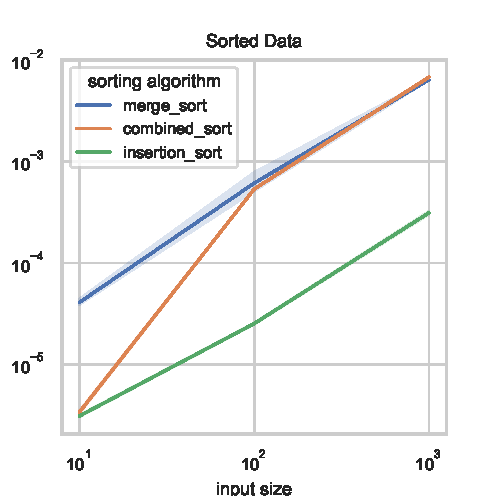
\includegraphics[width=0.8\columnwidth]{sorted_plot1000.pdf}
  % figure captions below figure
  \caption{Benchmark results sorted data, n=1000, log-log plot}
  \label{fig:bench}
\end{figure}



\vspace



\begin{figure}
  \centering
  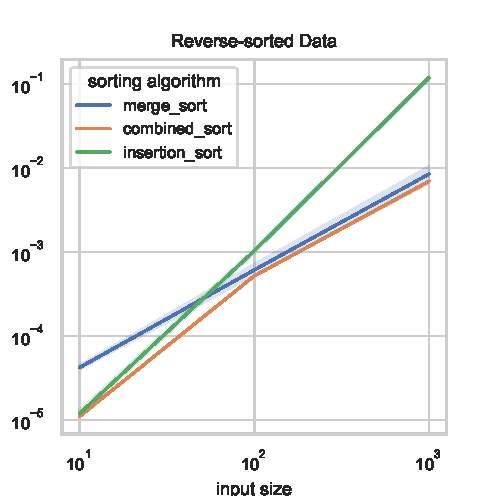
\includegraphics[width=0.8\columnwidth]{reversed_plot1000.pdf}
  % figure captions below figure
  \caption{Benchmark results reverse-sorted data, n=1000, log-log plot}
  \label{fig:bench}
\end{figure}

\begin{figure}
  \centering
  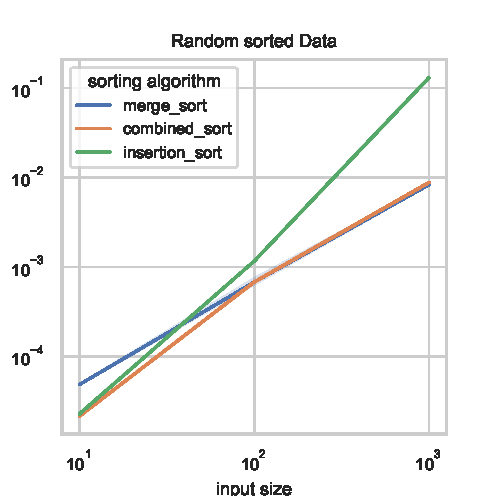
\includegraphics[width=0.8\columnwidth]{random_plot1000.pdf}
  % figure captions below figure
  \caption{Benchmark results random-sorted data, n=1000, log-log plot}
  \label{fig:bench}
\end{figure}


\section{Discussion}\label{sec:discussion}
The results after benchmarking sorting algorithms have showed that insertion-sort performs well on small sorted data while mergesort performs better if the number of elements exceed 100 and the data are either random, representing the average case or reversed-sorted representing the worst case. As the data size grows the performance of the two sorting-algorithms diverge, insertion-sort taking almost 20 times the amount used by mergesort in the worse case for 1000 elements. This is consistent with the theory, stating that in both worst- and average-case, the upper bound of the runtime of insertion-sort is quadratic in the input size. While in mergesort the runtime is, $ \theta (n lgn)$, with n representing the size of the input data. The combined algorithm will be a good compromise to achieve more flexibility. However its essential to know what threshold value should be used in advance to optimize performance. Our choice of threshold with data size equals 100 seems to be a bit too high. Overall however, considering the results carried out from this experiment, the performance of the combined algorithm is the best among the three candidates.





\section{Acknowledgements}\label{sec:acknowledgements}


\bibliographystyle{ACM-Reference-Format}
\bibliography{references.bib}

\end{document}